\documentclass{sig-alternate-ipsn13}

\begin{document}

\title{Estimating learning dynamics in the routing game
% \titlenote{}
}
%
% You need the command \numberofauthors to handle the 'placement
% and alignment' of the authors beneath the title.
%
% For aesthetic reasons, we recommend 'three authors at a time'
% i.e. three 'name/affiliation blocks' be placed beneath the title.
%
% NOTE: You are NOT restricted in how many 'rows' of
% "name/affiliations" may appear. We just ask that you restrict
% the number of 'columns' to three.
%
% Because of the available 'opening page real-estate'
% we ask you to refrain from putting more than six authors
% (two rows with three columns) beneath the article title.
% More than six makes the first-page appear very cluttered indeed.
%
% Use the \alignauthor commands to handle the names
% and affiliations for an 'aesthetic maximum' of six authors.
% Add names, affiliations, addresses for
% the seventh etc. author(s) as the argument for the
% \additionalauthors command.
% These 'additional authors' will be output/set for you
% without further effort on your part as the last section in
% the body of your article BEFORE References or any Appendices.

\numberofauthors{8} %  in this sample file, there are a *total*
% of EIGHT authors. SIX appear on the 'first-page' (for formatting
% reasons) and the remaining two appear in the \additionalauthors section.
%
\author{
% You can go ahead and credit any number of authors here,
% e.g. one 'row of three' or two rows (consisting of one row of three
% and a second row of one, two or three).
%
% The command \alignauthor (no curly braces needed) should
% precede each author name, affiliation/snail-mail address and
% e-mail address. Additionally, tag each line of
% affiliation/address with \affaddr, and tag the
% e-mail address with \email.
%
% 1st. author
% \alignauthor
% Ben Trovato\titlenote{Dr.~Trovato insisted his name be first.}\\
%        \affaddr{Institute for Clarity in Documentation}\\
%        \affaddr{1932 Wallamaloo Lane}\\
%        \affaddr{Wallamaloo, New Zealand}\\
%        \email{trovato@corporation.com}
% % 2nd. author
% \alignauthor
% G.K.M. Tobin\titlenote{The secretary disavows
% any knowledge of this author's actions.}\\
%        \affaddr{Institute for Clarity in Documentation}\\
%        \affaddr{P.O. Box 1212}\\
%        \affaddr{Dublin, Ohio 43017-6221}\\
%        \email{webmaster@marysville-ohio.com}
% % 3rd. author
% \alignauthor Lars Th{\o}rv{\"a}ld\titlenote{This author is the
% one who did all the really hard work.}\\
%        \affaddr{The Th{\o}rv{\"a}ld Group}\\
%        \affaddr{1 Th{\o}rv{\"a}ld Circle}\\
%        \affaddr{Hekla, Iceland}\\
%        \email{larst@affiliation.org}
% \and  % use '\and' if you need 'another row' of author names
% % 4th. author
% \alignauthor Lawrence P. Leipuner\\
%        \affaddr{Brookhaven Laboratories}\\
%        \affaddr{Brookhaven National Lab}\\
%        \affaddr{P.O. Box 5000}\\
%        \email{lleipuner@researchlabs.org}
% % 5th. author
% \alignauthor Sean Fogarty\\
%        \affaddr{NASA Ames Research Center}\\
%        \affaddr{Moffett Field}\\
%        \affaddr{California 94035}\\
%        \email{fogartys@amesres.org}
% % 6th. author
% \alignauthor Charles Palmer\\
%        \affaddr{Palmer Research Laboratories}\\
%        \affaddr{8600 Datapoint Drive}\\
%        \affaddr{San Antonio, Texas 78229}\\
%        \email{cpalmer@prl.com}
}
% There's nothing stopping you putting the seventh, eighth, etc.
% author on the opening page (as the 'third row') but we ask,
% for aesthetic reasons that you place these 'additional authors'
% in the \additional authors block, viz.
% \additionalauthors{Additional authors: John Smith (The Th{\o}rv{\"a}ld Group,
% email: {\texttt{jsmith@affiliation.org}}) and Julius P.~Kumquat
% (The Kumquat Consortium, email: {\texttt{jpkumquat@consortium.net}}).}
% \date{30 July 1999}
% Just remember to make sure that the TOTAL number of authors
% is the number that will appear on the first page PLUS the
% number that will appear in the \additionalauthors section.

\maketitle
\begin{abstract}

  The routing game models congestion on transportation and communication networks.
  We consider an online learning model of player dynamics: at each iteration, every player chooses an route (or a probability distribution over routes), then the joint decision of all players determines the costs of each path, which are then revealed to the players. We first review convergence guarantees of such online learning dynamics. Then, we consider the following estimation problem: given a sequence of player decisions and the corresponding costs, we would like to fit the learning model parameters to these observations. We consider in particular entropic mirror descent dynamics, and develop a numerical solution to the estimation problem.

  We demonstrate this method using data collected from a routing game experiment: we develop a web interface to simulate the routing game. When players log in to the interface, they are assigned an origin and destination on the graph. They can choose, at each iteration, a distribution over their available routes, and each player seeks to minimize her own cost. We collect a data set using this interface, then we apply the proposed method to fit the learning model parameters.
  We observe in particular that after an exploration phase, the joint decision of the players remains within a small distance of the Nash equilibrium. We also use the estimated model parameters to predict the flow distribution over routes, and compare these predictions to the actual distribution.
  Finally, we discuss some of the qualitative implications of these findings, and directions for future research.

\end{abstract}

\section{Introduction}

% Sections go here.  An example of figures is shown in Figure~\ref{fig:example}.

% \begin{figure}
% \centering
% 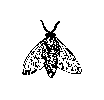
\epsfig{file=fly.eps}
% \caption{A sample black and white graphic (.eps format).}
% \label{fig:example}
% \end{figure}

\section{Experiment}

\subsection{I}

Two versions of the game were presented to the user. One version of the game allowed each player to select the flow distribution for each path, the other version of the game only allowed the player to choose an ``exploration'' parameter, which selects the flow distribution for the players based on the KL-divergence.
The players interfaced with the game through a web interface where they can enter their inputs and receive feedback of each of their path cost and the cumulative cost.


The cost for each player's distribution were normalized by the calculated equilibrium flow to account for imbalances in the network.


\subsection{II}
In the first version of the game, each player were allowed sliders to change how much of the flow are distributed to each path. All paths for a player have the same origin and destination node pair, but each player had unique origin and destination node pair.

\begin{figure}
  \centering
  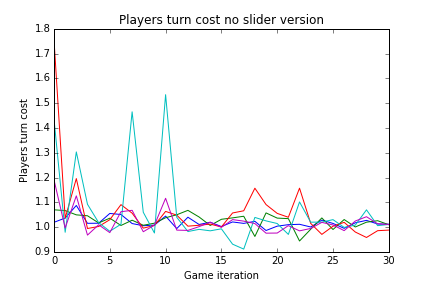
\includegraphics[width=80mm]{images/no_slider_players_costs.png}
  \caption{Player normalized cost for no slider version.}
  \label{fig:cost_no_slider}
\end{figure}


\begin{figure}
  \centering
  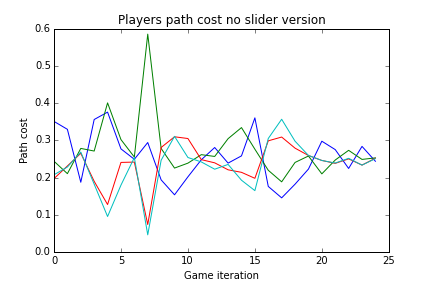
\includegraphics[width=80mm]{images/no_slider_path_costs.png}
  \caption{Predicted path cost.}
  \label{fig:predicted_path_cost}
\end{figure}


\begin{figure}
  \centering
  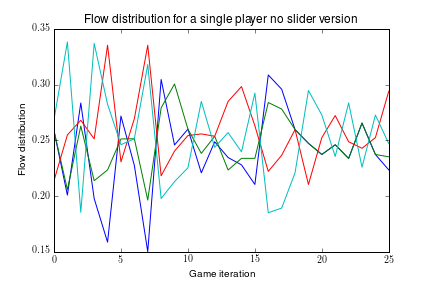
\includegraphics[width=80mm]{images/no_slider_actual_flow_distribution.png}
  \caption{Player flow distribution.}
  \label{fig:no_slider_player_flow_distribution}
\end{figure}

We estimate the learning rate, $\hat \eta^k_t$,  of the players at turn $t$ by

\[
  \hat \eta^k_t = \arg\min_{\eta \geq 0} D_{\psi_k}(\hat x_k^{(t+1)}(\eta), x^{(t+1)}_k)
\]


From these estimated learning rate sequence, we then estimate the flow distribution of iteration $t+1$ using $\hat \eta^k_t $ and $x_k^{(t)}$ with \ref{eq:KL_update}.


\subsection{III}

In the second version of the game, each player were only to change a single parameter $\eta$. This parameter controls how much each player want to explore from their previous flow distribution according to

\begin{equation} \label{eq:KL_update}
  (x_k^{(t+1)})_i = \frac{e^{-\eta_t^k (\ell^{(t)}_k)_i}}{\sum_j (x_k^{(t)})_i e^{-\eta_t^k (\ell^{(t)}_k)_i}}
\end{equation}

. The parameter for each turn is shown in \ref{fig:exploration}. We use a small $\epsilon$ to ensure that we will have no underflow for $x_k^{(t)}$ for numerical purposes. Then \ref{eq:KLupdate} becomes

\begin{equation} \label{eq:KL_update_epsilon}
  (x_k^{(t+1)})_i = \frac{e^{-\eta_t^k (\ell^{(t)}_k)_i}}{\sum_j (x_k^{(t)})_i e^{-\eta_t^k (\ell^{(t)}_k)_i}}
\end{equation}


\begin{figure}
  \centering
  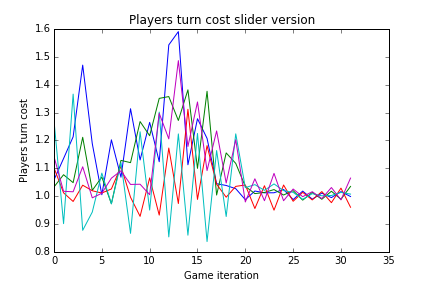
\includegraphics[width=80mm]{images/slider_players_costs.png}
  \caption{Player normalized cost for slider version.}
  \label{fig:cost_slider}
\end{figure}


\begin{figure}
  \centering
  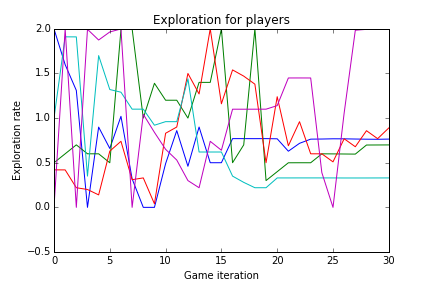
\includegraphics[width=80mm]{images/players_learning_rate.png}
  \caption{Player exploration rate.}
  \label{fig:exploration}
\end{figure}




% \begin{figure}
%   \centering
%   \includegraphics[width=80mm]{images/slider_path_costs.png}
%   \caption{Player exploration rate.}
%   \label{fig:exploration}
% \end{figure}


\section{Conclusions}
Conclusion goes here.

%ACKNOWLEDGMENTS are optional
\section*{Acknowledgments}
Acknowledgement goes here.

%
% The following two commands are all you need in the
% initial runs of your .tex file to
% produce the bibliography for the citations in your paper.
\bibliographystyle{abbrv}
\bibliography{sigproc}  % sigproc.bib is the name of the Bibliography in this case
% You must have a proper ".bib" file
%  and remember to run:
% latex bibtex latex latex
% to resolve all references
%
% ACM needs 'a single self-contained file'!
%
%APPENDICES are optional
%\balancecolumns
\appendix
%Appendix A

Appendix goes here.

% That's all folks!
\end{document}

%%% Local Variables:
%%% mode: latex
%%% TeX-master: t
%%% End:
